% theory and examples

\section{Fundamentals of Probability}

\subsection{Random Experiments}

\begin{example}
	\label{exmp:2.3.1}
	If we toss a coin, the outcome of the experiment will be tails, which we symbolize with the letter "T" or the number $0$, or heads, symbolized by $H$ or $1$—that is, one of the elements of the set $\set{T,H}$ (or $\set{0,1}.$)
\end{example}



\begin{example}
	\label{exmp:2.3.2}
	If we roll a die, the outcome of the experiment will result in one of the numbers from the set $\set{1,2,3,4,5,6}.$
\end{example}



\begin{example}
	\label{exmp:2.3.3}
	If we toss a coin twice, there are four possible outcomes:
	\begin{align}
		\set{HH,HT,TH,TT}.
	\end{align}
	
\end{example}



\begin{example}
	\label{exmp:2.3.4}
	If we are manufacturing screws with a machine, the outcome of the experiment is whether a screw comes out defective. Thus, once the screw is manufactured, it will belong to the set
	\begin{align}
		\set{\texttt{defective, not defective}}
	\end{align}
	
\end{example}



\begin{example}
	\label{exmp:2.3.5}
	If an experiment consists of measuring the \emph{lifespan} of an electric bulb produced by a company, then the outcome of the experiment is time $t$ measured in hours in some interval
	\begin{align}
		0\leq t \leq T,
	\end{align}
	where $T$ is the maximum lifetime of a bulb.
\end{example}



\subsection{The Sample Space}
A set $S$ consisting of all possible outcomes of a random experiment is called a \emph{sample space,} and each individual outcome is called a \emph{sample point.}

Usually, there will be more than one sample space that can describe an experiment, but we choose the one that provides the most useful information.

\begin{example}
	\label{exmp:2.3.6}
	If we roll a die, one possible sample space is given by $\set{1,2,3,4,5,6},$ whereas another is given by $\set{\text{even},\text{odd}}.$
\end{example}


\begin{example}
	\label{exmp:2.3.7}
	If we toss a coin twice consecutively, one possible sample space is given in Example \ref{exmp:2.3.3}, while another is given by
	\begin{align}
		\set{(0,0), (0,1), (1,0),(1,1)}.
	\end{align}
\end{example}



\begin{figure}
	\centering
	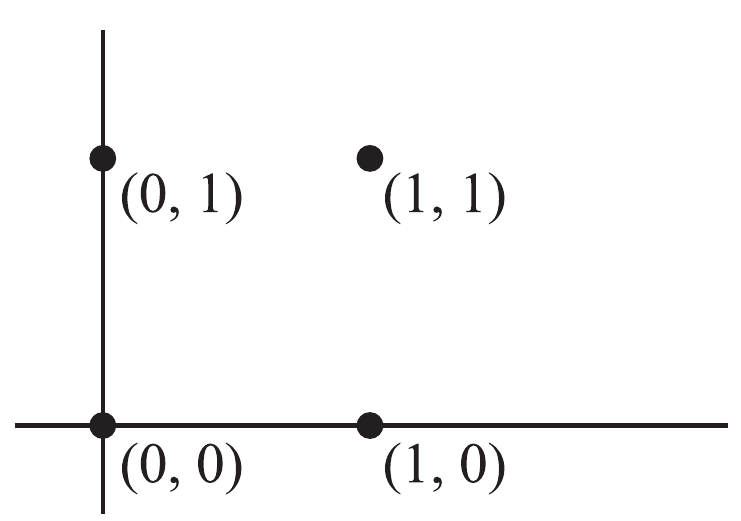
\includegraphics[width=5cm,keepaspectratio=true]{./pe/pands0101.png}
	% pands0101.png: 0x0 pixel, 300dpi, 0.00x0.00 cm, bb=
	\label{fig:2.3.1}
\end{figure}


{Types of Sample Spaces}
\begin{itemize}
	\item \emph{Finite:} Has a finite number of sample points.
	\item \emph{Countably infinite:} Has as many points as the natural numbers $\N$ (i.e., we can enumerate the space).
	\item \emph{Uncountably infinite:} Has as many points as the real line $\R.$ For instance, the interval $0<x<1.$
\end{itemize}



If the sample space is finite or countably infinite, we say it is \emph{discrete.} If it is uncountably infinite, we say it is \emph{continuous.}

\subsection{Events}

An \emph{event} is a subset $A$ of a sample space $S$—that is, a subset of all possible outcomes of an experiment. If the outcome is an element of $A,$ we say that \emph{$A$ has occurred.} 

An event consisting of a single sample point of $S$ is sometimes called an \emph{elementary or simple event.}


\begin{figure}
	\centering
	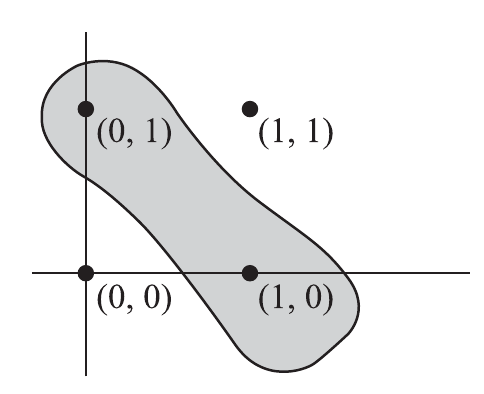
\includegraphics[height=3cm,keepaspectratio=true]{./pe/pands0102.png}
	% pands0102.png: 0x0 pixel, 300dpi, 0.00x0.00 cm, bb=
	\caption{Sample space for tossing a coin twice consecutively.}
	\label{fig:2.3.2}
\end{figure}



\begin{example}
	\label{exmp:2.3.8}
	If we toss a coin twice, the event that we obtain \emph{exactly} one tail is a subset of the sample space shown in Figure \ref{fig:2.3.2}.
\end{example}



As special cases, we can consider the entire sample space $S$ as the \emph{certain or sure event} and the empty set $\emptyset$ as the \emph{impossible event.}


\subsection{Operations Between Events} 
Suppose $A,B \subset S$ are two events. 
\begin{itemize}
	\item $A\cup B$ is the event \texttt{``$A$ or $B$ or both occur'',} and is also called the \emph{union of $A$ and $B$.}  
	\item $A\cap B$ is the event \texttt{``both $A$ and $B$ occur'',} and is also called the \emph{intersection of $A$ and $B$.}  
	\item $A'$ is the event \texttt{``$A$ does not occur'',} and is also called the \emph{complement or negation of $A$.} 
	\item $A-B=A\cap B'$ is the event \texttt{``$A$ occurs but $B$ does not'',} and is also called the \emph{difference of $A$ minus $B.$} Notice that
	$A' = S - A.$
\end{itemize}


If $A\cap B= \emptyset,$ then we say that $A$ and $B$ are \emph{disjoint} or \emph{mutuarly exclusive.} 

\begin{definition}
	If $A_{1},A_{2},... \subset S$ is a collection of events such that $A_{i}\cap A_{j}=\emptyset$ whenever $i\neq j,$ then we say they are \emph{mutuarly exclusive events}.
\end{definition}

\begin{definition}
	If $A_{1}, A_{2}, ...\subset S$ are mutually exclusive events, we say that $A_{1} \cup A_{2} \cup ... $ is the \emph{disjoint union} of such events, and in that case we write
	\begin{align}
		A_{1}\sqcup A_{2} \sqcup ...
	\end{align}
\end{definition}


\begin{definition}
	If \begin{align}
		S=A_{1}\sqcup A_{2} \sqcup ...
	\end{align}
	we say that $A_{1},A_{2},...\subset S$ is a \emph{partition of $S.$}
\end{definition}


\begin{example}
	\label{exmp:2.3.9}
	Regarding the experiment of tossing a coin twice, consider the event $A$ consisting of \emph{obtaining at least one head,} while event $B$ consists of \emph{the second toss being a tail.}
	
	Then $A=\set{TH,HT,HH},$ $B=\set{HT,TT}$ and therefore:
	\begin{enumerate}
		\item $A\cup B =$ $\set{HT,TH,HH,TT}= S$ 
		\item $A\cap B =$ $\set{HT}$ 
		\item $A'=$$\set{TT}$
		\item $A-B=$$\set{TH,HH}$
	\end{enumerate}
	
\end{example}


\subsection{Approaches to Probability}

Any event in a sample space can be assigned a number between $0=0\%$ and $1=100\%$ representing its \emph{probability} of occurring.


If an event can occur in $h$ different ways out of a total of $n$ possible outcomes, all equally plausible, then the probability of the event is $h/n.$


\begin{example}
	\label{exmp:2.3.10}
	Suppose we want to know the probability that heads appears on a single coin toss. Since there are two \emph{equally likely} different ways the coin can land, and out of those two ways heads can occur in only one way, we reason that its probability is $1/2.$
	
	
	\begin{remark}
		Here we assume that the coin is fair and unbiased.
	\end{remark}
	
\end{example}


If after $n$ repetitions of an experiment, where $n$ is sufficiently large, an event is observed to occur $h$ times, then we say that the probability of the event is $h/n.$ This is also called the \emph{empirical probability} of the event.


\begin{example}
	\label{exmp:2.3.11}
	If we toss a coin $1000$ times and obtain heads 532 times, we estimate the resulting probability to be $532/1000=0.532$.
\end{example}



\begin{remark}
	Both approaches have their limitations:
	\begin{enumerate}
		\item In the classical case, the phrase \emph{``equally likely''} is somewhat circular and vague; 
		\item whereas in the frequentist approach, \emph{``a very large number''} is not mathematically precise. 
	\end{enumerate}
	For these reasons, mathematicians have developed an \emph{axiomatic approach} to probability.
\end{remark}


\subsection{The Axioms of Probability}

Suppose we have a sample space $S.$ Let $C$ be the collection of all events in $S.$ We say that $P:C \to \R$ is a probability function if it satisfies the following properties:

\begin{axiom}
	For every event $A,$ we have
	\begin{align}
		\label{eq:2.3.1}
		P(A)\geq 0.
	\end{align}
	
\end{axiom}



\begin{axiom}
	The probability of the certain event $S$ is
	\begin{align}
		\label{eq:2.3.2}
		P(S)=1.
	\end{align}
\end{axiom}



\begin{axiom}
	For any countable sequence of mutually exclusive events $A_{1},A_{2},...$ we have
	\begin{align}
		\label{eq:2.3.3}
		P(A_{1}\sqcup A_{2} \sqcup ...)=P(A_{1})+P(A_{2})+...
	\end{align}
	In particular, for two mutually exclusive events $A_{1},A_{2},$
	\begin{align}
		\label{eq:2.3.4}
		P(A_{1}\sqcup A_{2})=P(A_{1})+P(A_{2})
	\end{align}
	
\end{axiom}


\subsection{Some Important Theorems in Probability}

\begin{theorem}
	\label{thm:2.3.1}
	If $A_{1}\subset A_{2},$ then $P(A_{1})\leq P(A_{2})$ and
	\begin{align}
		P(A_{2}-A_{1})=P(A_{2})-P(A_{1}).
	\end{align}
\end{theorem}

\begin{proof}
	Since $A_1 \subset A_2$, we can write $A_2 = A_1 \cup (A_2 - A_1)$ where $A_1$ and $A_2 - A_1$ are disjoint.
	
	By Axiom 3:
	\begin{align}
		P(A_2) &= P(A_1 \cup (A_2 - A_1)) \\
		&= P(A_1) + P(A_2 - A_1)
	\end{align}
	
	Since $P(A_2 - A_1) \geq 0$ (Axiom 1), it follows that $P(A_1) \leq P(A_2)$.
	
	Solving for the difference: $P(A_2 - A_1) = P(A_2) - P(A_1)$.
\end{proof}


\begin{theorem}
	\label{thm:2.3.2}
	For every event $A$,
	\begin{align}
		\label{eq:2.3.5}
		0\leq P(A) \leq 1,
	\end{align}
	
	that is, probability always lies between $0\%$ and $100\%.$
\end{theorem}

\begin{proof}
	The inequality $P(A) \geq 0$ follows directly from Axiom 1.
	
	To prove $P(A) \leq 1$, observe that $A \subset S$, so applying Theorem \ref{thm:2.3.1}:
	\begin{align}
		P(A) \leq P(S) = 1
	\end{align}
	by Axiom 2.
\end{proof}


\begin{theorem}
	\label{thm:2.3.3}
	The impossible event has zero probability, that is,
	\begin{align}
		P(\emptyset)=0.
	\end{align}
\end{theorem}

\begin{proof}
	Since $\emptyset \subset S$ and $\emptyset \cap S = \emptyset$, we can write $S = S \cup \emptyset$ as a disjoint union.
	
	By Axiom 3:
	\begin{align}
		P(S) &= P(S \cup \emptyset) = P(S) + P(\emptyset)
	\end{align}
	
	Since $P(S) = 1$ (Axiom 2), we have:
	\begin{align}
		1 = 1 + P(\emptyset) \implies P(\emptyset) = 0
	\end{align}
\end{proof}


\begin{theorem}
	\label{thm:2.3.4} The probability of the complementary event is given by
	\begin{align}
		\label{eq:2.3.6}
		P(A')=1-P(A)
	\end{align}
\end{theorem}

\begin{proof}
	Since $A$ and $A'$ are disjoint and $A \cup A' = S$, by Axiom 3:
	\begin{align}
		P(S) &= P(A \cup A') = P(A) + P(A')
	\end{align}
	
	Since $P(S) = 1$ (Axiom 2), solving for $P(A')$ yields:
	\begin{align}
		P(A') = 1 - P(A)
	\end{align}
\end{proof}

\begin{theorem}
	\label{thm:2.3.5} If $A=A_{1}\sqcup...\sqcup A_{N}$ is the disjoint union of mutually exclusive events, then
	\begin{align}
		\label{eq:2.3.7}
		P(A)=P(A_{1})+...+P(A_{N}).
	\end{align}


	In particular, if $S=A_{1}\sqcup...\sqcup A_{N}$ then
	\begin{align}
		\label{eq:2.3.8}
		P(A_{1})+...+P(A_{N})=1.
	\end{align}
\end{theorem}


\begin{theorem}
	\label{thm:2.3.6}
	If $A,B,C$ are events that are not necessarily mutually exclusive, then
	\begin{align}
		\label{eq:2.3.9}
		P(A\cup B)=P(A)+P(B)-P(A\cap B).
	\end{align}
	\begin{align}
		\label{eq:2.3.10}
		P(A\cup B \cup C)&=P(A)+P(B)+P(C)\\
		&-P(A\cap B)-P(B\cap C)-P(C\cap A)\\
		&+P(A\cap B \cap C).
	\end{align}
\end{theorem}



\begin{theorem}
	\label{thm:2.3.7}
	For any events $A,B,$
	\begin{align}
		\label{eq:2.3.11}
		P(A)=P(A\cap B)+P(A\cap B').
	\end{align}
\end{theorem}



\begin{theorem}
	\label{thm:2.3.8}
	If $A_{1},A_{2},..., A_{N}$ form a partition of the sample space $S,$ that is,
	$S=A_{1} \sqcup A_{2} \sqcup ... \sqcup A_{N},$ then for any event $A$
	\begin{align}
		\label{eq:2.3.12}
		P(A)=P(A\cap A_{1})+ P(A\cap A_{2}) + ... +P(A\cap A_{N}).
	\end{align}
\end{theorem}


\subsection{Assignment of Probabilities}

If a sample space consists of a \emph{finite} number of possible outcomes $a_{1},...,a_{N},$ then by Theorem \ref{thm:2.3.5},
\begin{align}
	\label{eq:2.3.13}
	P(A_{1})+...+P(A_{n})=1
\end{align}
where $A_{1},...,A_{n}$ are \emph{elementary sets} or \emph{simple events} given by $A_{i}=\set{a_{i}}.$


It follows that one can arbitrarily choose any non-negative numbers as probabilities of these simple events, provided that \eqref{eq:2.3.13} is satisfied.

In particular, if we assume \emph{equal probabilities} for all simple events, then
\begin{align}
	\label{eq:2.3.14}
	P(A_{k})=\dfrac{1}{n}, \; k=1,2,...,n,
\end{align}
and if $A$ is an event formed by the disjoint union of $h$ simple events, then
\begin{align}
	\label{eq:2.3.15}
	P(A)=\dfrac{h}{n}.
\end{align}


\begin{remark}
	This is equivalent to the \textit{classical approach.} But we can also use the \textit{frequentist approach} to assign these probabilities.
\end{remark}


\begin{example}
	\label{exmp:2.3.12}
	If a single die is rolled, the probability that we obtain either a 2 or a 5 is 
	\[ P(\set{2,5}) = P(\set{2}) + P(\{5\}) = 1/6 + 1/6 = 1/3. \]
\end{example}
